\chapter{Attuatori e pianta completa}
\section{Modello nominale}
La coppia richiesta dal controllore non viene applicata direttamente alla dinamica SEA. Per rappresentare banda finita e latenza, ogni canale è descritto da un secondo ordine a guadagno statico unitario seguito da un ritardo di trasporto:
\[
\bar G_m(s)=\frac{\bar\omega_n^2}{s^2+2\bar\zeta\bar\omega_n s+\bar\omega_n^2}e^{-\bar\tau_ds},
\]
con $\bar\omega_n=\ActuatorWn$ rad/s, $\bar\zeta=\ActuatorZeta$ e $\bar\tau_d=\ActuatorDelayMs$ ms. Questi valori non sono dati identificati: sono stati selezionati fra 27 combinazioni di frequenza naturale, smorzamento e ritardo. I criteri richiedono una banda sensibilmente maggiore dei modi instabili a bassa frequenza, ma inferiore ai primi modi elastici; impongono inoltre overshoot del singolo attuatore non superiore al 2\% e un errore di fase Padé moderato a 80 rad/s.

La combinazione scelta, $40$ rad/s, $0.8$ e $15$ ms, fornisce una banda di circa $34.78$ rad/s. È quindi abbastanza rapida rispetto ai poli instabili a 4.04 e 7.21 s$^{-1}$, mentre inizia a filtrare il comando prima delle risonanze elastiche a circa 70--79 rad/s. Lo smorzamento $0.8$ limita la sovraelongazione senza imporre una dinamica criticamente smorzata; il ritardo di 15 ms rimane non trascurabile e viene incluso esplicitamente.

\section{Approssimazione del ritardo}
La traccia richiede un Padé del primo ordine:
\[
e^{-\tau_ds}\simeq \frac{1-\tau_ds/2}{1+\tau_ds/2}.
\]
L'approssimazione aggiunge un polo stabile in $-2/\tau_d$ e uno zero nel semipiano destro in $+2/\tau_d$. Lo zero è conseguenza della rappresentazione razionale del ritardo e rende il canale non minimum-phase, ma non introduce un polo instabile. L'errore di fase è trascurabile in prossimità dei modi instabili meccanici e cresce avvicinandosi ai modi elastici; il modello non deve quindi essere extrapolato indiscriminatamente alle alte frequenze.
\begin{figure}[H]\centering
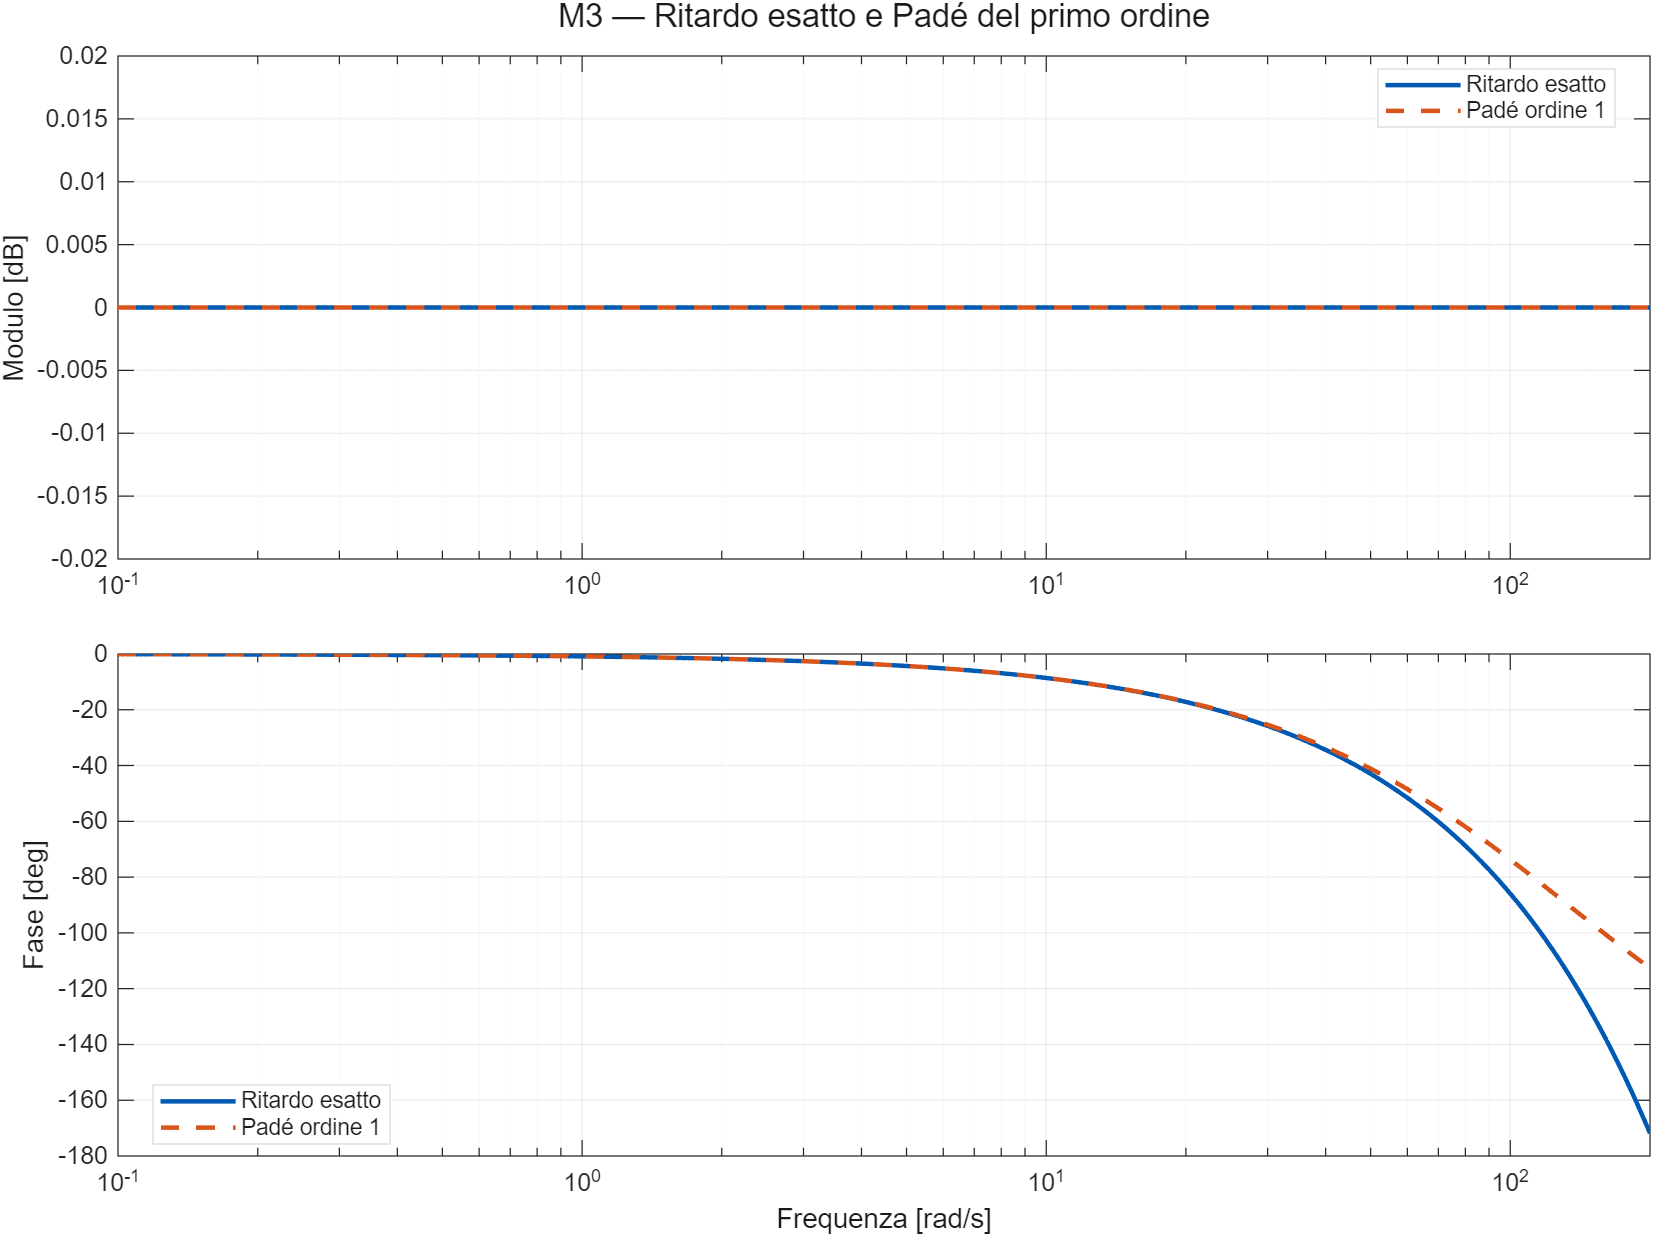
\includegraphics[width=0.76\textwidth]{figures/m3_delay_pade_comparison.png}
\caption{Confronto fra ritardo esatto e Padé del primo ordine (M3).}\label{fig:m3-pade}
\end{figure}

\section{Interconnessione con la meccanica}
Ogni attuatore razionale ha ordine tre; due copie diagonali aggiungono sei stati agli otto stati meccanici. La pianta nominale completa ha quindi ordine \FullPlantOrder. Indicando con $(A_a,B_a,C_a,D_a)$ la realizzazione dei due attuatori e con $(A_m,B_m,C_m,D_m)$ la meccanica, la cascata è costruita esplicitamente per preservare l'ordine degli stati:
\[
A_{full}=\begin{bmatrix}A_m&B_mC_a\\0&A_a\end{bmatrix},\qquad
B_{full}=\begin{bmatrix}B_mD_a\\B_a\end{bmatrix}.
\]
Il comando $u$ attraversa la dinamica attuativa e produce la coppia motore $\tau$. Le coppie di disturbo fisiche introdotte in seguito agiscono invece direttamente sul lato link, evitando di confondere un carico esterno con un errore del comando. La costruzione è stata confrontata in frequenza con una cascata indipendente e coincide entro la precisione numerica.

La pianta completa conserva i due poli meccanici instabili e aggiunge soltanto poli attuativi stabili. Dopo un opportuno scaling temporale, i test SVD e PBH confermano controllabilità e osservabilità dei 14 stati. L'ordine completo viene mantenuto nelle sintesi: non sono effettuate cancellazioni dei modi elastici o dello zero Padé.
